A l'issue de la phase d'analyse, le code est disponible sous la forme d'une liste de \pyinline{StructureNode} (figure \ref{fig:parse_exemple}). C'est à partir de cette liste que sera produit le code assembleur et le code binaire associé.

L'ensemble des classes décrites ci-dessous font l'objet d'un transtypage permettant d'afficher celles-ci sous la forme d'une chaîne de caractères. 

\subsubsection{Classe StructureNode}

\begin{figure}
	\centering
	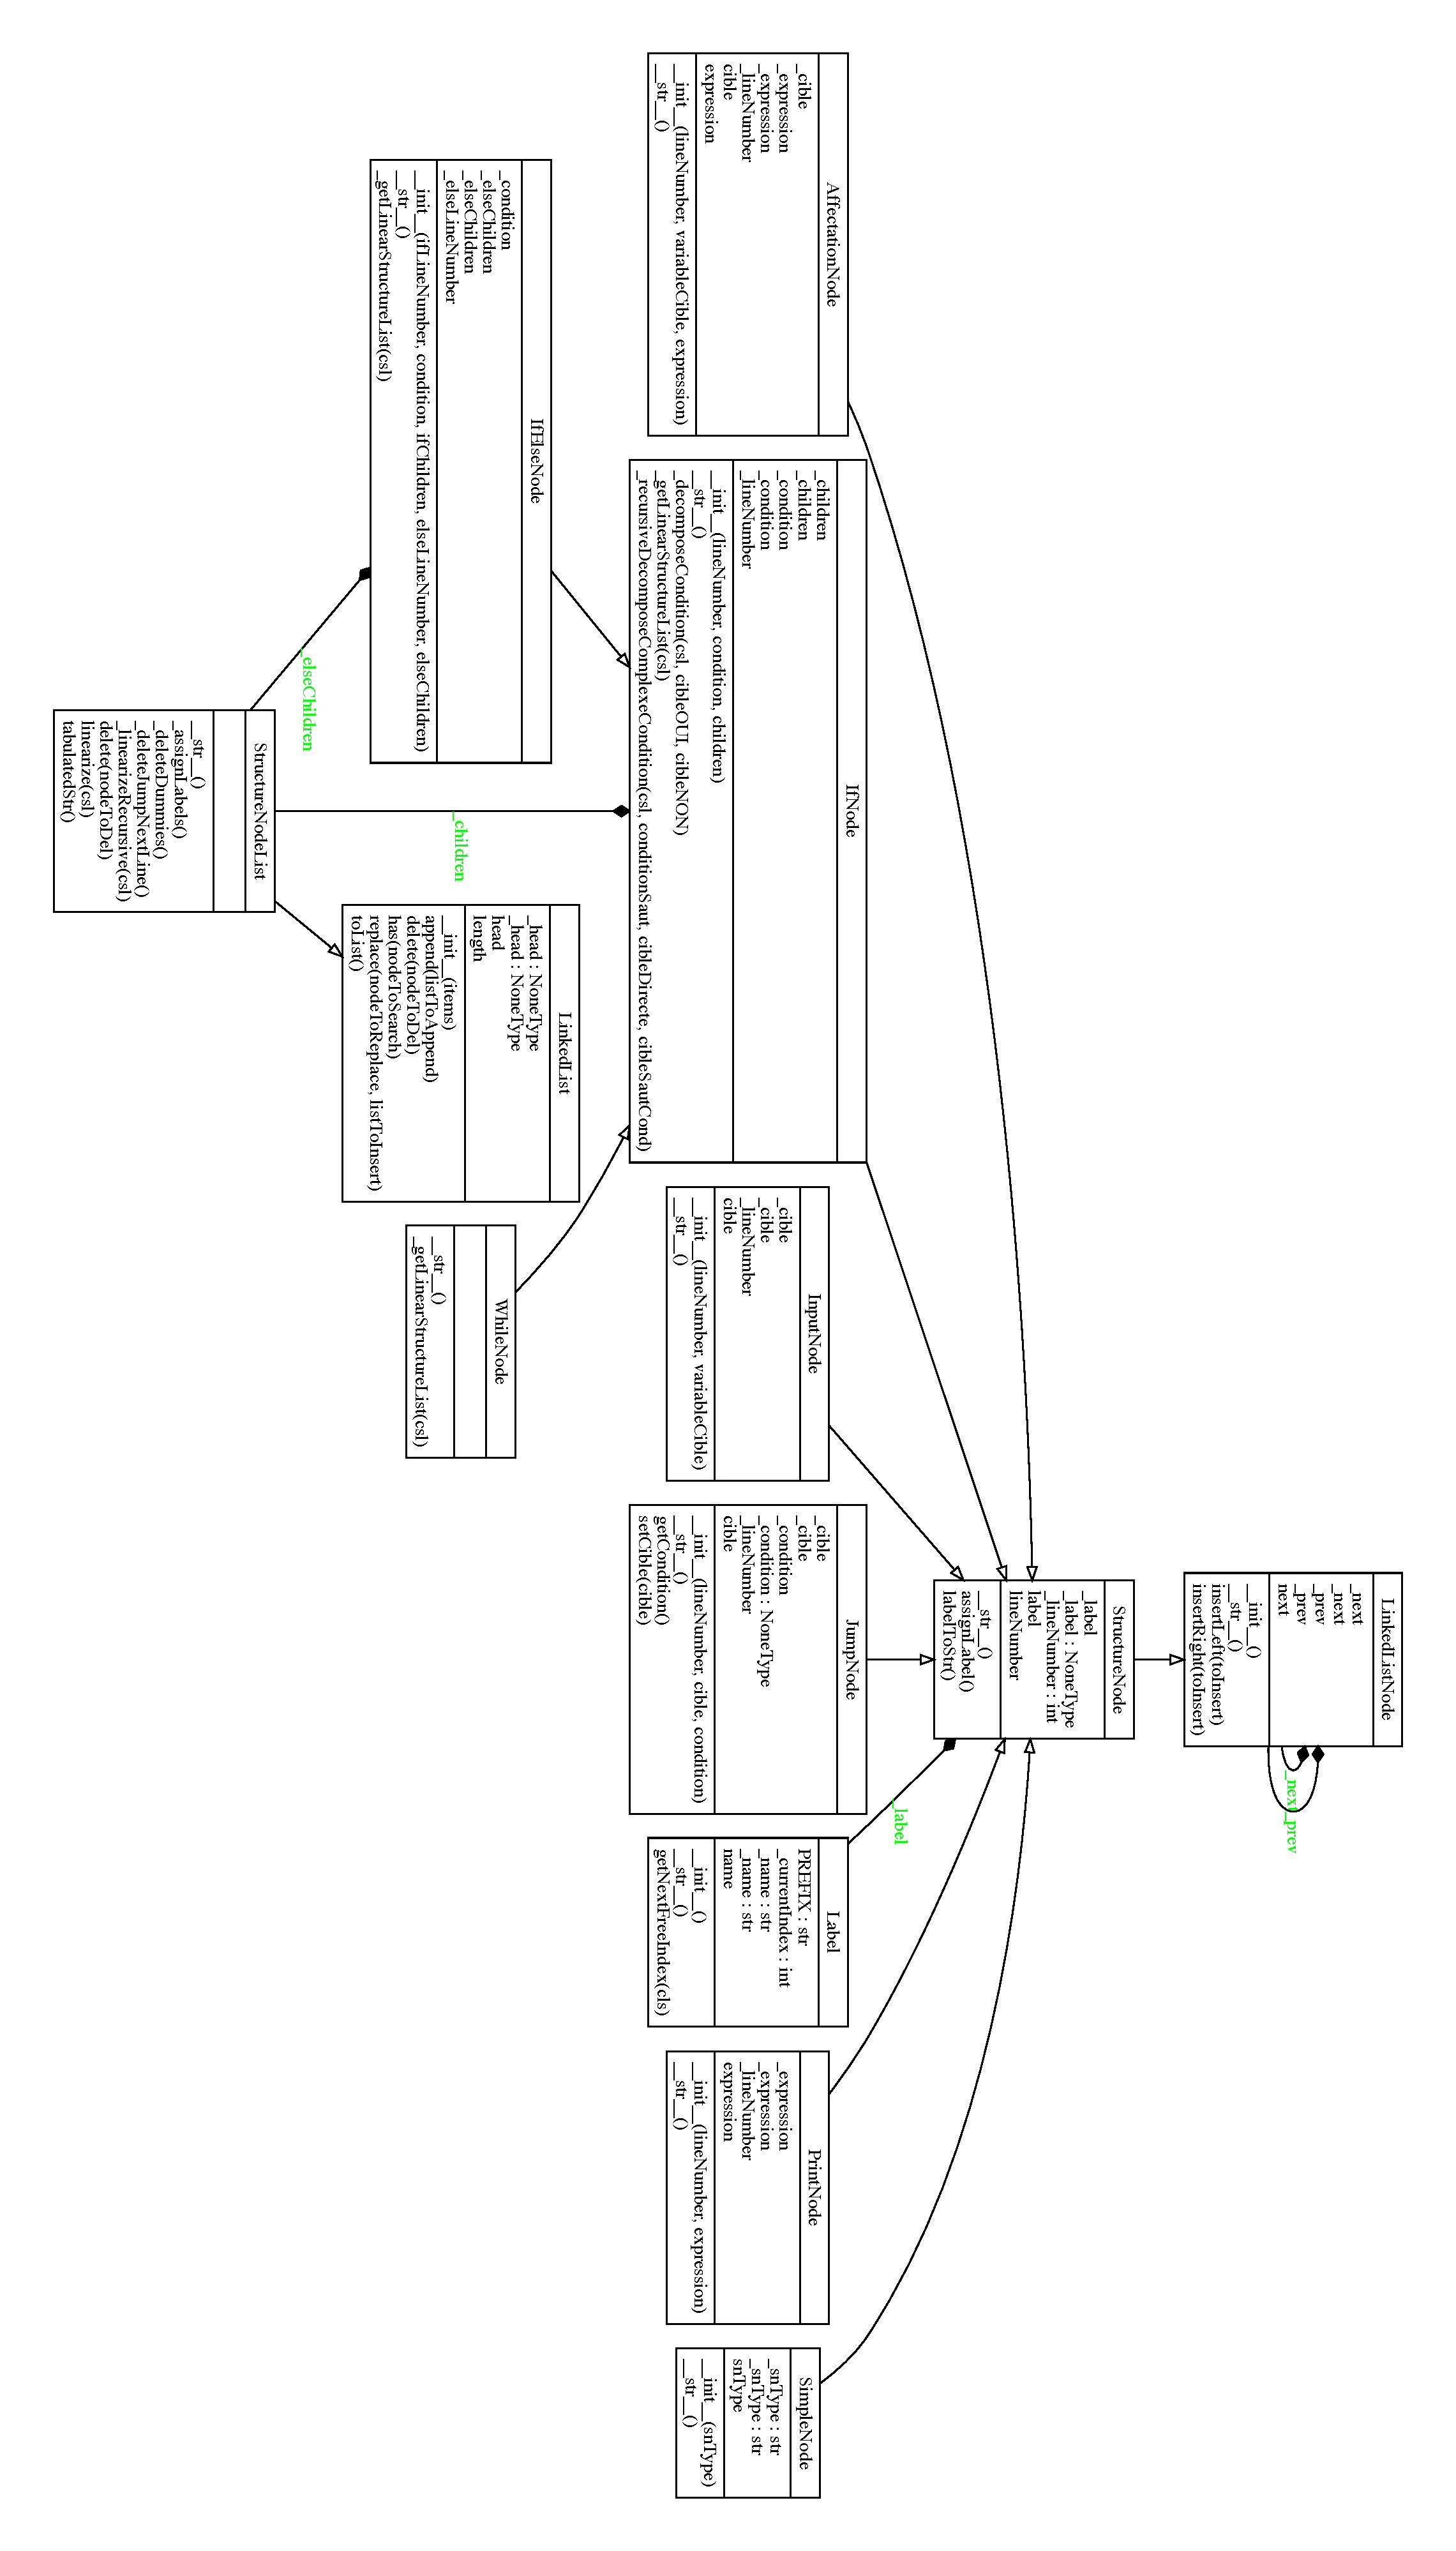
\includegraphics[height=25cm]{./Pictures/StructureNode.pdf}
	\caption{\label{fig:class_StructureNode}Diagramme de classes - StructureNode}
\end{figure}

Les classes héritées de \pyinline{StructureNode} sont présentées sur la figure \ref{fig:class_StructureNode}. On remarquera que les \pyinline{StructureNode} peuvent être des structures de données récursives, les n\oe uds de type \pyinline{IfNode}, \pyinline{IfElseNode} et \pyinline{WhileNode} ayant pour attribut \pyinline{_children} de type \pyinline{StructureNodeList}.
\clearpage

\subsubsection{Classes ArithmeticExpressionNode, LogicExpressionNode et ComparisonExpressionNode}

Les conditions de branchement \pyinline{if ... then} ou d'arrêt de boucle \pyinline{while} sont implémentées comme attribut (\pyinline{_condition}) des n\oe uds de type \pyinline{IfNode}, \pyinline{IfElseNode} et \pyinline{WhileNode}. Elles sont associées à des instances des classes \pyinline{LogicExpressionNode} ou \pyinline{ComparisonExpressionNode}.

\begin{figure}[h!]
	\centering
	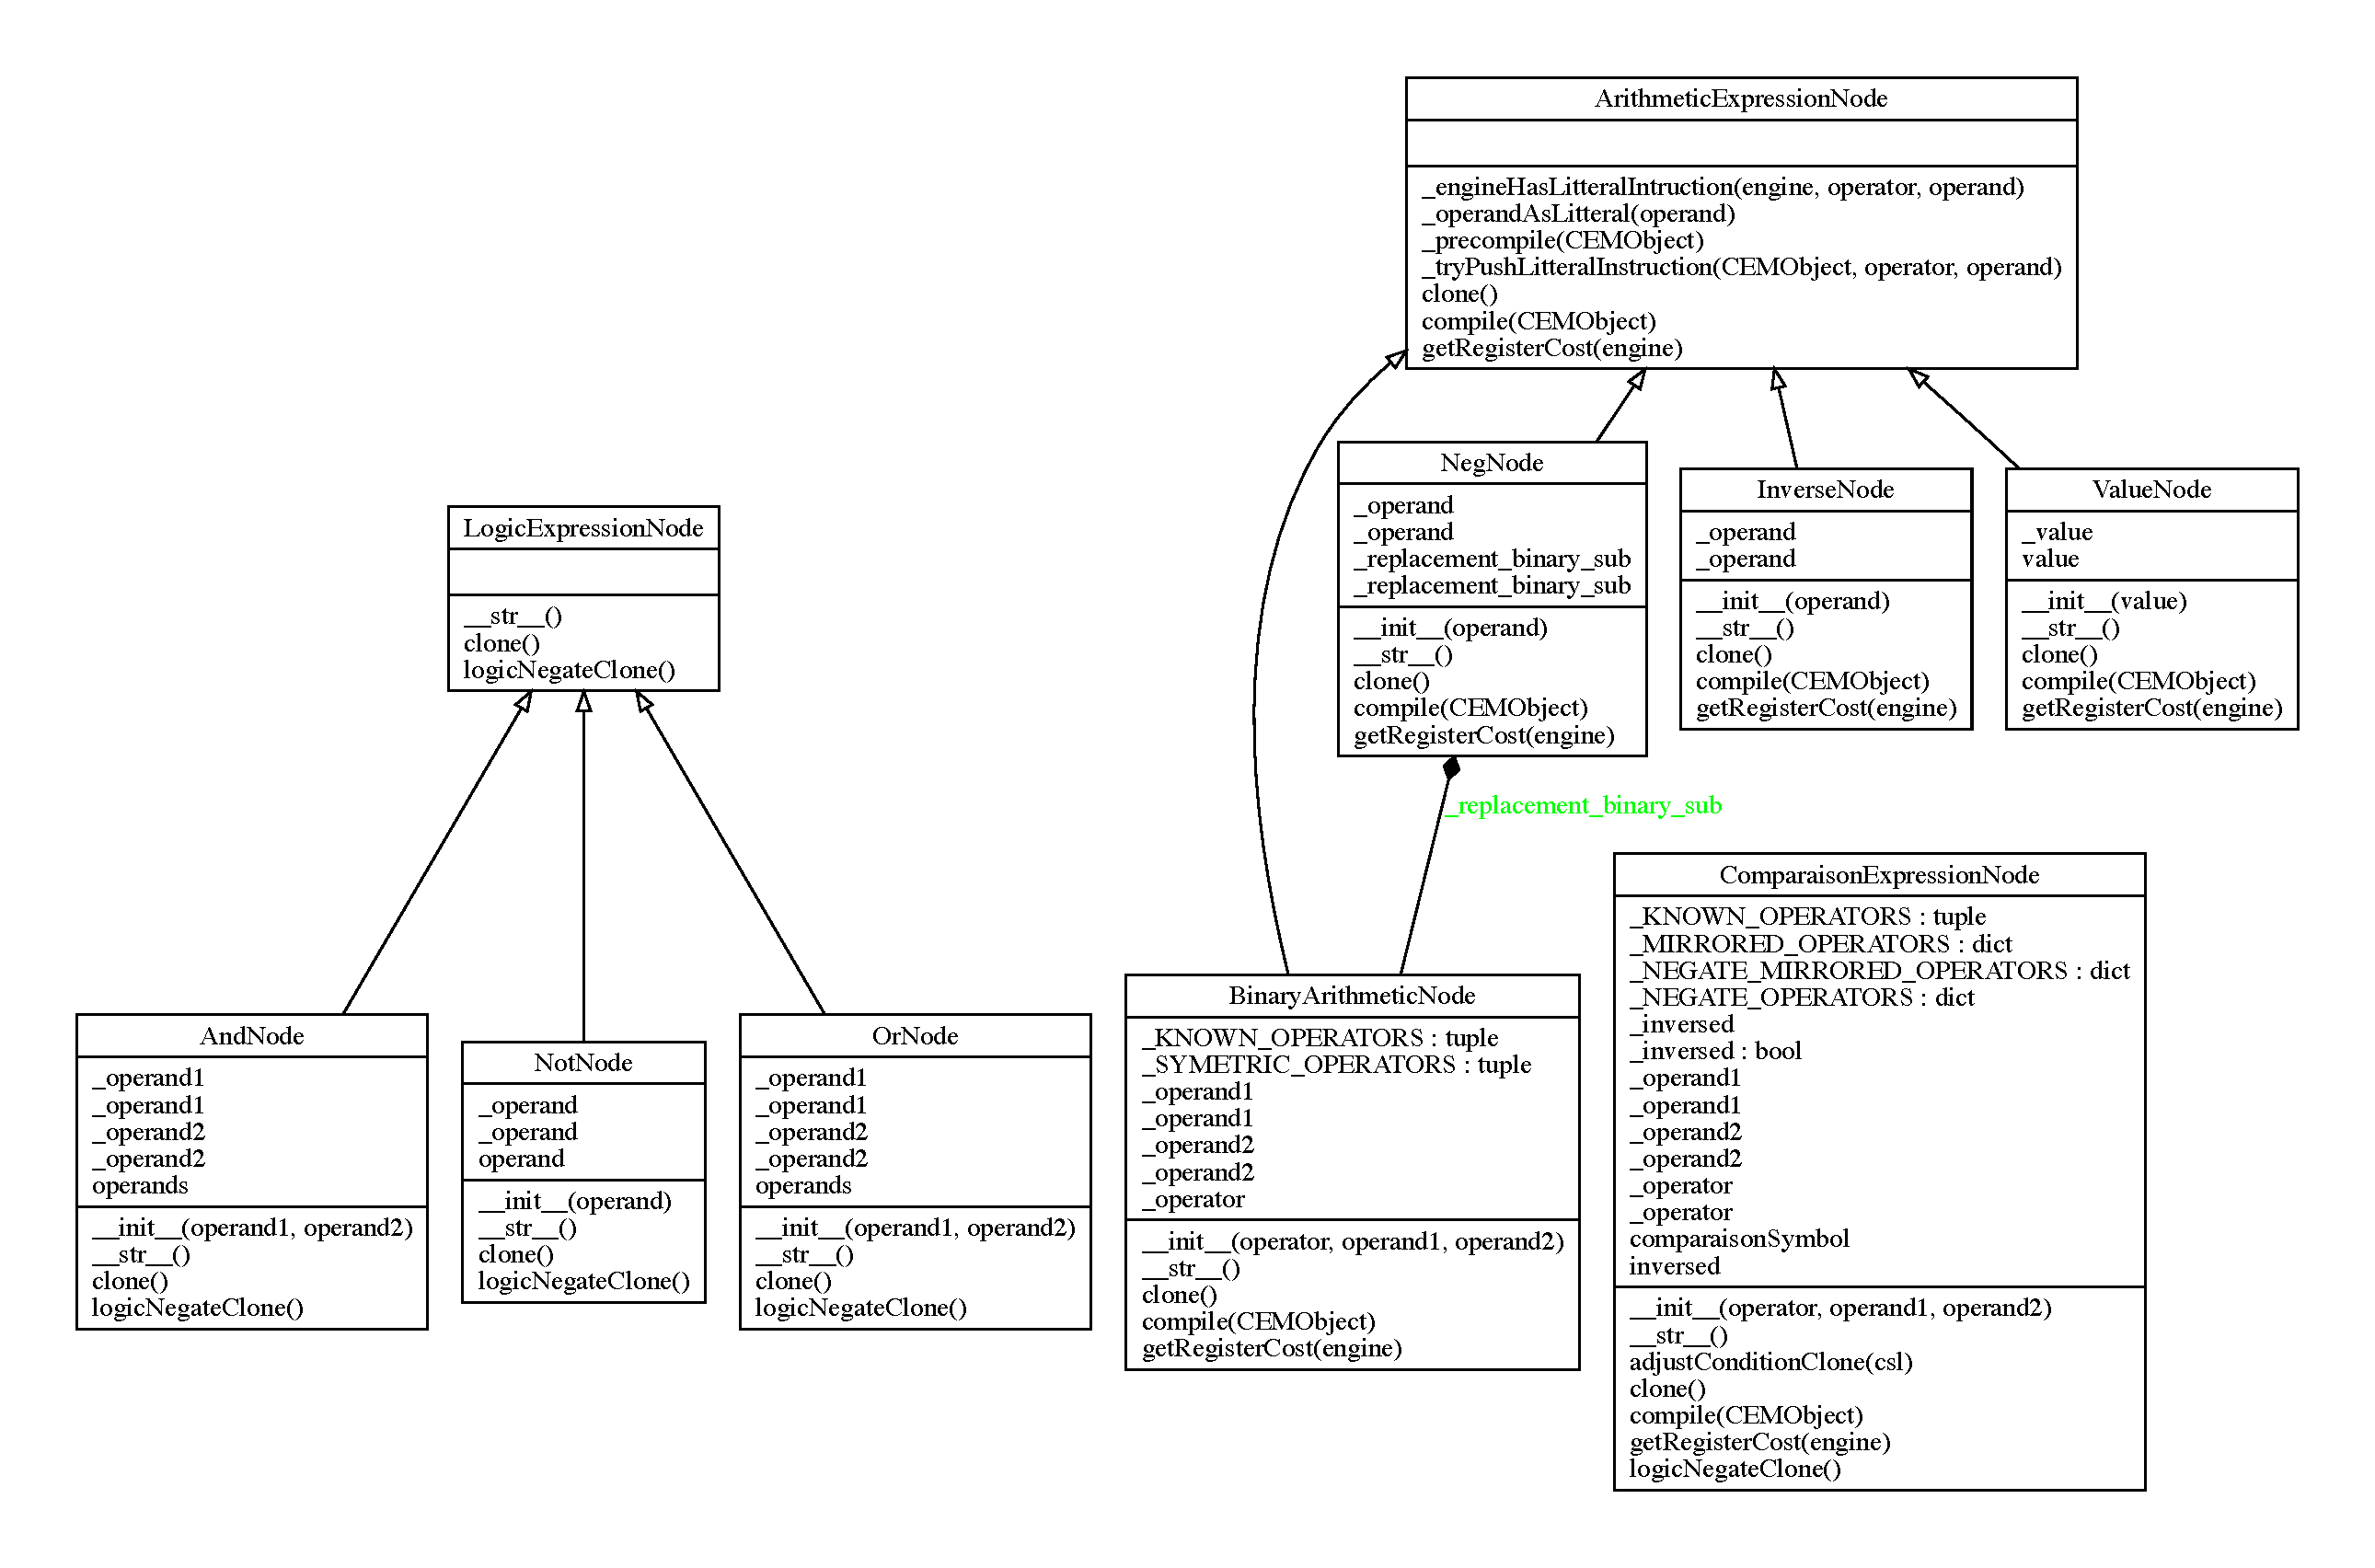
\includegraphics[width=\textwidth]{./Pictures/ExpressionNode.pdf}
	\caption{\label{fig:class_ExpressionNode}Diagramme de classes - ExpressionNode}
\end{figure}

Les expressions de type comparaisons (\pyinline{ComparisonExpressionNode}), expression arithmétiques \pyinline{ArithmeticExpressionNode} ou les affectations (\pyinline{AffectationNode}) peuvent avoir pour attributs des instances de la classe \pyinline{ArithmeticExpressionNode}.